\documentclass[a4paper,12pt]{article}
\usepackage[utf8]{inputenc}

%  Русский язык
\usepackage{multirow}
\usepackage{wrapfig}
\usepackage[T2A]{fontenc}			% кодировка
\usepackage[utf8]{inputenc}			% кодировка исходного текста
\usepackage[english,russian]{babel}	% локализация и переносы

\usepackage{indentfirst} %Красная строка
\usepackage[a4paper,top=1.3cm,bottom=2cm,left=1.5cm,right=1.5cm,marginparwidth=0.5cm]{geometry}
\usepackage[usenames]{color}
\usepackage{colortbl}
\usepackage{csvsimple}
\usepackage{siunitx}

\addto\captionsrussian{\def\refname{5   Список используемой литературы}}

% Заметки
\usepackage{todonotes}

% Математика
\usepackage{amsmath,amsfonts,amssymb,amsthm,mathtools} 
\usepackage{hyperref}

\renewcommand{\AA}{\ensuremath{\mathring{A}}}

\begin{document}
\def\figurename{Рисунок}
\begin{titlepage}
\begin{center}
    {\large МОСКОВСКИЙ ФИЗИКО-ТЕХНИЧЕСКИЙ ИНСТИТУТ (НАЦИОНАЛЬНЫЙ ИССЛЕДОВАТЕЛЬСКИЙ УНИВЕРСИТЕТ)}
\end{center}
\begin{center}
    {\largeФизтех-школа биологической и медицинской физики}
\end{center}

\vspace{1cm}
{\huge
\begin{center}
    {\bf Лабораторная работа по оптике}\\
    \vspace{0.5cm}
    4.7.3. Поляризация.
\end{center}
}

\vspace{4cm}
\begin{flushright}
{\LARGE Выполнила студентка группы Б06-103:\\ Фитэль Алена \\}

\end{flushright}
\vspace{9cm}
\begin{center}
    Долгопрудный, 2023 г.
\end{center}
\end{titlepage}
\newpage


\section{Аннотация}

\textbf{Цель работы:} ознакомление с методами получения и анализа поляризованного света.

\textbf{Приборы и материалы:} оптическая скамья с осветителем, зеленый светофильтр, два поляроида, черное зеркало, полированная эбонитовая пластинка, стопа стеклянных пластинок, слюдяные пластинки разной толщины, пластинки в 1/4 и 1/2 длины волны, пластинка в одну длину волны для зеленого света.


\section{Теоретические сведения}

\subsection{Определение направления разрешённой плоскости колебаний поляроида}
	
	Определить направление разрешённых колебаний поляроида проще всего с помощью чёрного зеркала.
	
При падении света на отражающую поверхность под углом Брюстера, свет в отражённом луче почти полностью поляризован, а вектор E
параллелен отражающей поверхности ("<правило иголки">). Луч света,
прошедший поляроид и отразившийся от чёрного зеркала, имеет минимальную интенсивность при выполнении двух условий: во-первых, свет
падает на отражающую поверхность под углом Брюстера и, во-вторых,
в падающем пучке вектор E лежит в плоскости падения.

Вращая поляроид вокруг направления луча и чёрное зеркало вокруг
оси, перпендикулярной лучу, методом последовательных приближений
можно добиться минимальной яркости луча, отражённого от зеркала,
и таким образом определить разрешённое направление поляроида.

Измеряя угол поворота зеркала (угол Брюстера), нетрудно определить коэффициент преломления материала, из которого изготовлено
зеркало. Описанный метод часто используется для измерения коэффициента преломления непрозрачных диэлектриков.

\subsection{Получение эллиптически поляризованного света}


\begin{figure}[h!]
    \centering
    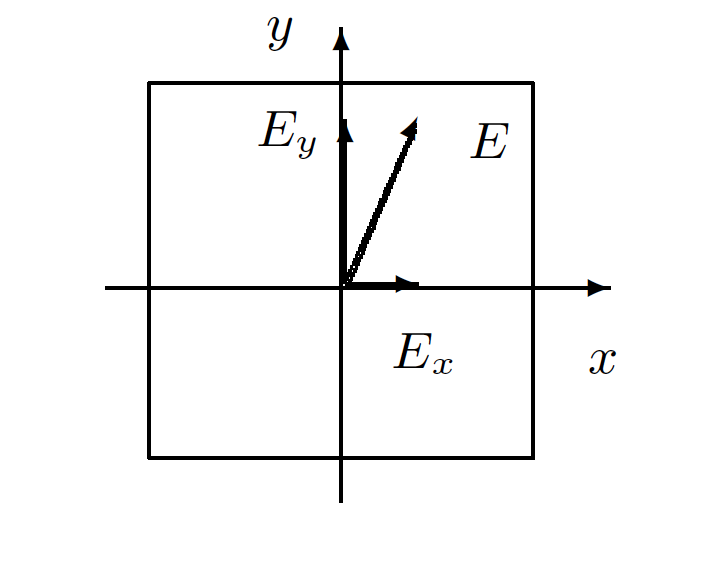
\includegraphics[scale = 0.4]{1 (1).png}
    \caption{Разложение линейно поляризованного света по главным направлениям двоякопреломляющей пластинки }
    \label{fig : 1}
\end{figure}


Эллиптически поляризованный свет можно получить из линейно поляризованного с
помощью двоякопреломляющих кристаллических пластинок.

Двоякопреломляющая пластинка имеет два взаимно перпендикулярных главных направления, совпадающих с осями эллипсоида диэлектрической проницаемости. Волны, поляризованные вдоль главных направлений, распространяются в пластинке с разными скоростями, не изменяя характера своей поляризации. Эти волны называются главными. Мы будем обозначать показатели преломления для главных волн через $ n_x $ и $ n_y $, где $ x $ и $ y $ --- главные направления кристаллической пластинки (рис. 1).

Пусть на пластинку падает линейно поляризованная волна, электрический вектор которой ориентирован под некоторым углом $ \alpha $ к оси
$ x $. Разложим вектор $ \mathbf{E} $ на составляющие $ E_x $ и $ E_y $. На входе пластинки $ E_x $ и $ E_y $ находятся в фазе. На выходе из-за разности скоростей между ними появляется разность хода $ d(n_x - n_y) $, при этом сдвиг фаз определяется соотношением

\begin{equation}\label{}
\Delta \phi =  \dfrac{2\pi}{m} = k d(n_x - n_y)
\end{equation}
Как уже отмечалось, при сложении двух взаимно перпендикулярных колебаний, обладающих некоторым сдвигом фаз, образуется колебание, поляризованное по эллипсу.


\begin{figure}[h!]
    \centering
    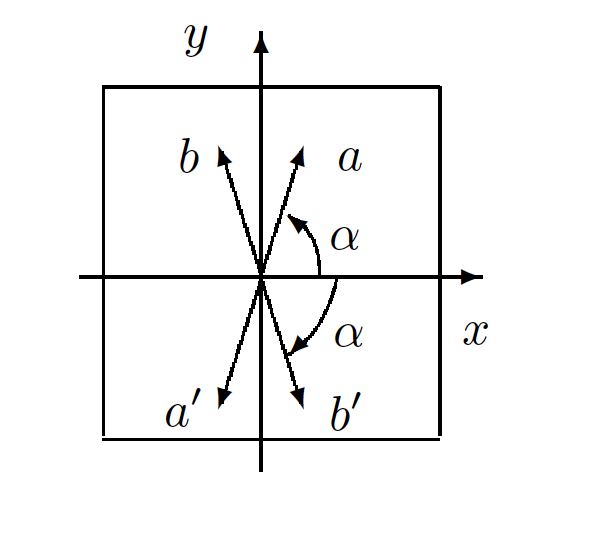
\includegraphics[scale = 0.4]{2.png}
    \caption{Поворот направления колебаний с помощью пластинки в $ \lambda / 2 $}
    \label{fig : 1}
\end{figure}

Рассмотрим практически важные частные случаи.

 \begin{enumerate}
 		
 	\item Пластинка даёт сдвиг фаз $ 2\pi $ (пластинка в длину волны $ \lambda $). В результате сложения волн на выходе пластинки образует-
ся линейно поляризованная волна с тем же направлением колебаний, что и в падающей волне.

	\item Пластинка даёт сдвиг фаз $ \pi $ (пластинка в полдлины волны $ \lambda / 2 $). На выходе пластинки снова образуется линейно поляризованная волна. Направление $ bb' $ колебаний этой волны повёрнуто относительно направления $ aa' $ колебаний падающей волны (рис. 2). Как нетрудно сообразить, направление $ bb' $ является зеркальным отображением направления $ aa' $ относительно одного из главных направлений пластинки. Такую пластинку используют для поворота направления колебаний линейно поляризованного света.
	
	\item Пластинка создаёт между колебаниями сдвиг фаз $ \pi/2 $ (пластинка
в четверть длины волны). При сложении двух взаимно перпендикулярных колебаний, имеющих разность фаз $ \pi/2 $, образуется эллипс, главные оси которого совпадают с координатными осями $ x $ и $ y $. При равенстве амплитуд возникает круговая поляризация.
 	
 \end{enumerate}

Следует отметить, что, говоря о пластинках $ \lambda , \lambda/2, \lambda/4  $ и т. д., всегда подразумевают какую-либо вполне определённую монохроматическую
компоненту (например, пластинка $ \lambda/2 $ для зелёного света). Если на двоякопреломляющую пластинку падает не монохроматический свет, то на
выходе из неё для разных спектральных компонент эллипсы поляризации будут различными.

\subsection{Анализ эллиптически поляризованного света}

Анализ эллиптически поляризованного света сводится к нахождению главных осей
эллипса поляризации и к определению направления вращения электрического вектора.

Главные оси эллипса поляризации определяются с помощью анализатора по максимуму и минимуму интенсивности проходящего света.
Направление вращения электрического вектора может быть найдено
с помощью пластинки в четверть длины волны, для которой известно,
какая из главных волн, $ E_x $ или $ E_y $, имеет б\'{o}льшую скорость распространения (и соответственно меньшее значение показателя преломления).

Выберем для определённости координатные оси x и y на пластинке
так, чтобы $ nx < ny $. В этом случае главная волна $ E_x $ имеет большую
скорость распространения. Поместим такую пластинку на пути эллиптически поляризованного света и совместим главные направления пластинки $ \lambda/4 $ с главными осями эллипса поляризации. На выходе из этой
пластинки сдвиг фаз между $ E_x $ и $ E_y $ вместо $ \pi/2 $ станет равным ну-
лю или $ \pi $. Свет окажется линейно поляризованным. Из двух возможных значений сдвига фаз, 0 или $ \pi $, реализуется одно: то, которое соответствует имеющемуся в волне направлению вращения электрического вектора.

Рассмотрим, например, случай, когда электрический вектор в эллиптически поляризованной волне вращается против часовой стрелки,
если смотреть навстречу лучу. В этом случае, очевидно, в волне, падающей на пластинку в $ \lambda/4 $, колебание $ E_y $ отстаёт по фазе на $ \pi/2 $ от
колебания $ E_x $. При прохождении через пластинку разность фаз увеличивается до $ \pi $. Таким образом на выходе из пластинки возникают линейно поляризованные волны со сдвигом фаз $ \pi $. Сложение этих волн
даёт плоскополяризованную волну, электрический вектор которой рас-
полагается во втором и четвёртом квадрантах координатной системы
$ x, y $.

Рассуждая аналогичным образом, найдём, что при вращении электрического вектора по часовой стрелке направление колебаний в линейно поляризованной волне, выходящей из пластинки, располагается в первом и третьем квадрантах. Определяя направление колебаний на выходе из пластинки с помощью поляроида, можно, таким образом, определить характер эллиптической поляризации (вращение против или по часовой стрелке).


\begin{figure}[h!]
    \centering
    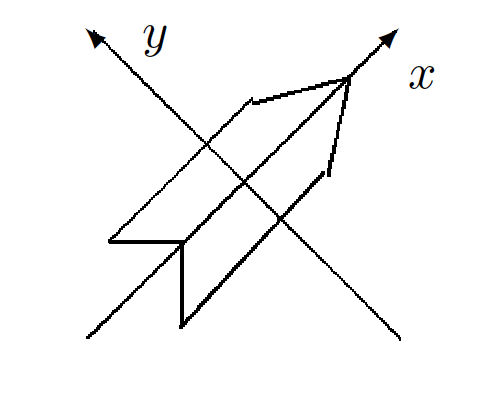
\includegraphics[scale = 0.4]{3.png}
    \caption{Пластинка чувствительного оттенка}
    \label{fig : 1}
\end{figure}
Выше предполагалось известным, какому из двух главных направлений пластинки в четверть длины волны соответствует большая скорость распространения света.
Установить это можно различными способами, например с помощью
пластинки чувствительного оттенка (так называют пластинку в $ \lambda $
для зелёной спектральной компоненты, $ \lambda = 560 $ нм).

Пластинка имеет форму стрелы (рис. 3), вдоль оси которой расположено главное направление, соответствующее большей скорости распространения.

Если пластинка чувствительного оттенка помещена между скрещенными поляроидами и главные направления пластинки не параллельны
направлениям разрешённых колебаний поляроидов, то при освещении
белым светом пластинка кажется окрашенной в лилово-красный цвет.
Это объясняется тем, что зелёная компонента линейно поляризованного света при прохождении пластинки не меняет поляризации и задерживается вторым поляроидом. Для красной и фиолетовой компонент
пластинка создаёт сдвиг фаз, несколько отличный от $ 2\pi $. На выходе
из пластинки красная и фиолетовая компоненты оказываются поэтому
эллиптически поляризованными и частично проходят через второй поляроид. Таким образом, в известном смысле наблюдаемый в указанном
опыте цвет пластинки дополнителен к зелёному.

Если между скрещенными поляроидами поместить пластинку чувствительного оттенка
($ \lambda $) и пластинку в $ \lambda/4 $ так, чтобы их главные
направления совпадали, цвет пластинки изменится. Если у пластинки чувствительного оттенка и пластинки в $ \lambda/4  $совпадут главные направления, соответствующие большей скорости распространения, то разность хода между $ E_x $ и $ E_y $ для зелёного света составит уже $ 5\lambda/4 $. Это соответствует разности хода в $ \lambda $ для света с большей длиной волны, т. е. для "<более красного"> света. При освещении
этих пластинок (напомним, что они расположены между скрещенными поляроидами) белым светом теперь погасится не зелёная, а красная
часть спектра, и проходящий свет будет казаться зеленовато-голубым.
Если же главные направления, соответствующие большей скорости распространения, у пластинки чувствительного оттенка и у пластинки
в $ \lambda/4 $ окажутся перпендикулярными, то проходящий свет приобретёт
оранжево-желтую окраску (погасится фиолетово-голубая часть спектра).

Изменение цвета позволяет, таким образом, определить, какое из
главных направлений пластинки в $ \lambda/4 $ соответствует большей скорости
распространения.

\subsection{Интерференция поляризованных лучей}


\begin{figure}[h!]
    \centering
    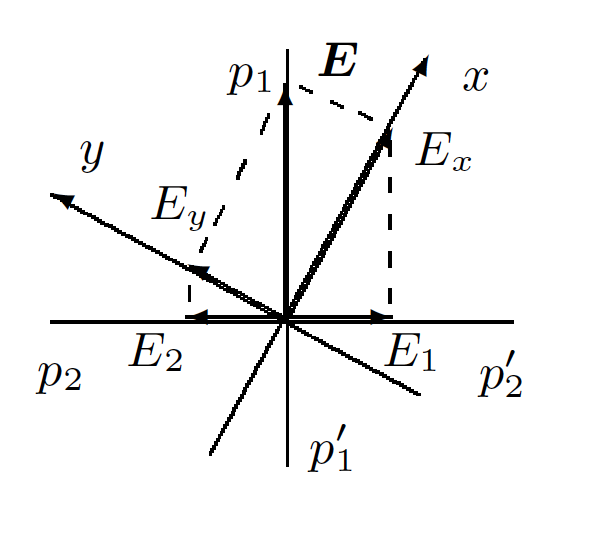
\includegraphics[scale = 0.4]{4.png}
    \caption{К объяснению интерференции поляризованных лучей}
    \label{fig : 1}
\end{figure}

Тонкие двоякопреломляющие пластинки, помещённые между поляроидами, кажутся окрашенными. Эта окраска может быть истолкована как результат интерференции поляризованных лучей. На рис. 4 представлена схема для
случая скрещенных поляроидов.

Здесь $ p1p'1 $ --- разрешённое направление колебаний поляризатора
(первого поляроида); $ x, y $ --- координатная система, связанная с главны-
ми направлениями двоякопреломляющей пластинки; $ p2p'2 $ --- разрешённое направление колебаний анализатора (второго поляроида). Волны
$ E_x  $ и $ E_y $ на выходе из пластинки когерентны, но не могут интерферировать, так как $ E_x \perp  E_y $. Волны $ E_1 $ и $ E_2 $ на выходе второго поляроида
также являются когерентными и к тому же поляризованы в одной плоскости. Эти волны интерферируют между собой. Результат интерференции определяется зависящим от длины волны сдвигом фаз между $ E_1 $
и $ E_2 $. В результате интерференции поляризованных лучей пластинка, освещаемая белым светом, кажется окрашенной.

Если поворачивать двоякопреломляющую пластинку, расположенную между
скрещенными поляроидами, то соотношение амплитуд волн $ E_1 $ и $ E_2 $ и разность фаз между ними не изменяются. Это означает, что цвет пластинки при её поворотах не меняется, а меняется только интенсивность света. За один оборот пластинки интенсивность четыре раза обращается в нуль --- это происходит при совпадении главных направлений
$ x $ и $ y $ с разрешёнными направлениями колебаний поляроидов.

Если же двоякопреломляющую пластинку оставить неподвижной, а
второй поляроид повернуть так, чтобы разрешённые направления $ p1p'1 $
и $ p2p'2 $ совпали, то волны $ E_1 $ и $ E_2 $ приобретают дополнительный фазовый сдвиг на $ \pi $ для всех спектральных компонент; при этом их амплитуды изменятся так, что цвет пластинки изменится на дополнительный. 

\section{Ход работы}

\subsection{Определение разрешенных направлений поляроида}



\begin{figure}[h!]
    \centering
    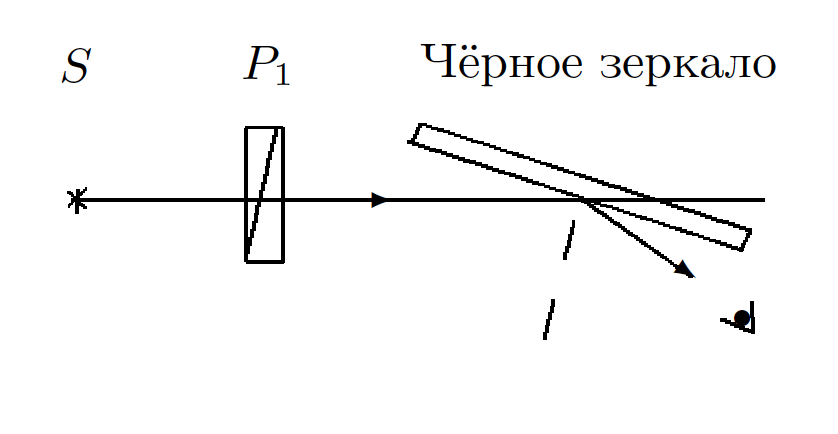
\includegraphics[scale = 0.6]{5.png}
    \caption{Определение разрешенных направлений поляроида}
    \label{fig : 1}
\end{figure}
Поворачивая поляроид вокруг направления луча, а чёрное зеркало вокруг вертикальной оси, методом последовательных приближений добьемся
наименьшей яркости отражённого пятна (Рисунок 5). Для первого поляроида угол поворота $\alpha_p^1 = 176^\circ\pm2^\circ$.

Определить направление второго поляроида можно по схеме, изображенной на Рисунке 6. 


\begin{figure}[h!]
    \centering
    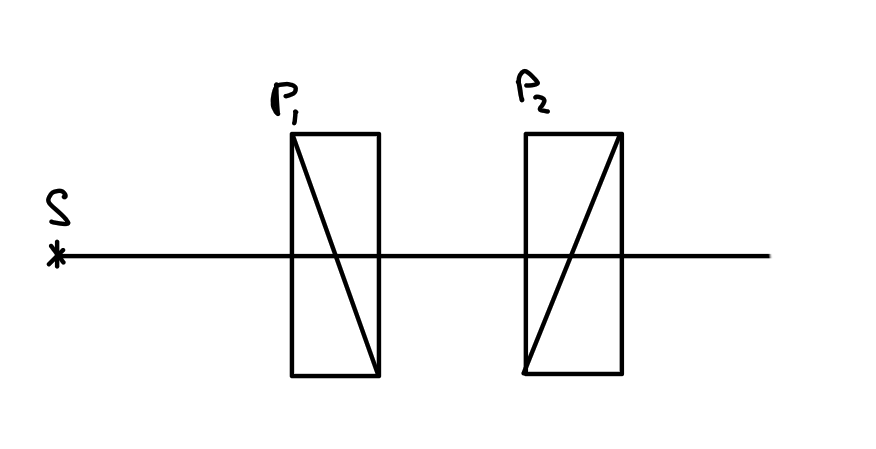
\includegraphics[scale = 0.8]{9.png}
    \caption{Определение разрешенного  направления второго поляроида}
    \label{fig : 1}
\end{figure}

Интенсивность будет минимальна, если разрешенное направление 2-го поляроида будет перпендикулярно первому. Это происходит при угле $\alpha_p^2=120^\circ\pm1^\circ$.

\subsection{Определение коэффициента преломления эбонита}
Теперь определим угол Брюстера для эбонита. Воспользуемся схемой аналогичной Рисунку 5, только вместо зеркала расположим эбонитовую пластину. Запишем показания лимба в перпендикулярном положении и под углом Брюстера.

\begin{table}[h!]
	\centering
	\begin{tabular}{|c|c|c|}
		\hline
		$\alpha^0$            & $\alpha^1$            & $\varphi_B = \alpha^1-\alpha^0$ \\ \hline
		$179^\circ\pm1^\circ$ & $238^\circ\pm1^\circ$ & $59^\circ\pm1,2^\circ$            \\ \hline
	\end{tabular}
\end{table}
Для измерений с фильтром результаты оказались теми же.

Показатель преломления $n$ посчитаем так
\[
	n = \tan{\varphi_B} = 1,66\pm0,07
\]

Табличное значение показателя преломления эбонита: $n = 1,6-1,7$.


\subsection{Исследование стопы}

\begin{figure}[h!]
    \centering
    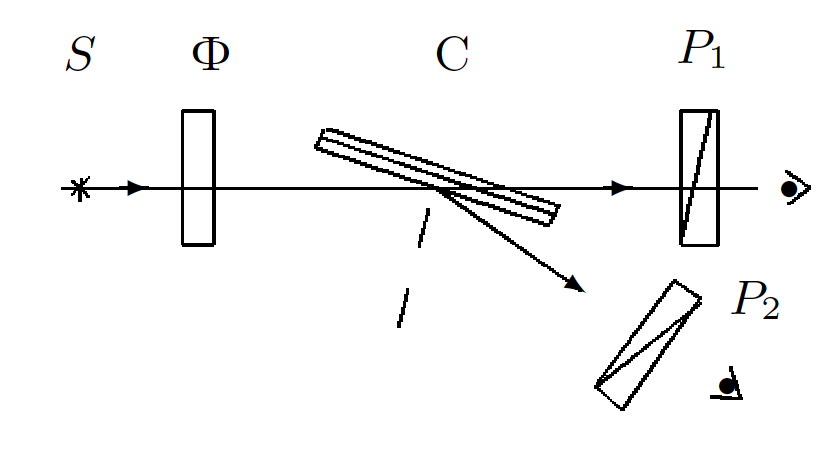
\includegraphics[scale = 0.4]{6.png}
    \caption{Исследование стопы}
    \label{fig : 1}
\end{figure}


Исследуем характер поляризации света в преломлённом и отражённом от стопы лучах.  Для этого поставим вместо эбонитового зеркала (Рисунок 7) стопу стеклянных пластинок под углом Брюстера. С помощью поляроида можно увидеть, что отраженный свет имеет вертикальную поляризацию. При рассматривании прошедшего луча, при повороте поляроида заметны перепады яркости, но свет никогда не исчезает полностью. Это значит, что есть не линейно поляризованная составляющая.

\subsection{Двоякопреломляющие пластины}

Определим главные направления двоякопреломляющих пластин. 
\begin{figure}[h!]
    \centering
    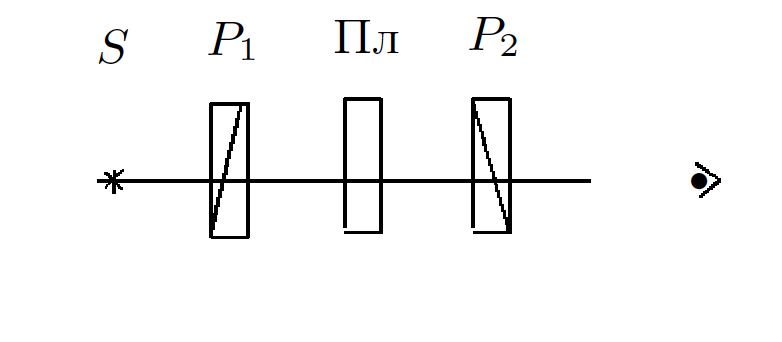
\includegraphics[scale = 0.4]{7.png}
    \caption{Определение главных
		направлений в пластинках}
    \label{fig : 1}
\end{figure}

Поставим кристаллическую пластинку между скрещенными поляроидами (Рисунок 8). Вращая пластинку будем наблюдать за минимумами интенсивности прошедшего света. В этом случае главные направления пластинки совпадут с разрешенными направлениями поляроидов. 


	
	Пластинка 1:
	\[
		\alpha_1^1 = 110^\circ
	\]
	\[
		\alpha_1^2 = 20^\circ
	\]
	Видно, что направления взаимно перпендикулярны.
	
	Пластинка 2:
	\[
	\alpha_2^1 = 261^\circ
	\]
	\[
	\alpha_2^2 = 171^\circ
	\]


\subsection{Пластинки $ \lambda/2, \lambda/4 $}

Добавим к предыдущей схеме зеленый фильтр и развернем исследуемую пластинку под $45^\circ$ относительно осей поляроидов. Теперь, вращая анализатор определим характер поляризации.
	
	Пластинка 1: Линейная поляризация, а значит это пластинка $\lambda/2$.
	
	Пластинка 2: Круговая поляризация, а значит это пластинка $\lambda/4$.
	

\subsection{Быстрая и медленная оси $ \lambda/4 $}.


\begin{figure}[h!]
    \centering
    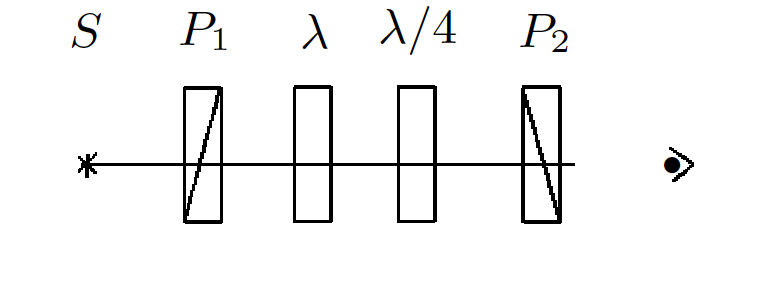
\includegraphics[scale = 0.4]{8.png}
    \caption{Определение направлений
большей и меньшей скорости}
    \label{fig : 1}
\end{figure}



Определим "<быструю"> и "<медленную"> оси в пластинке $ \lambda/4 $.

Поставим между скрещенными поляроидами пластинку чувствительного оттенка, имеющую вид стрелки, и убедимся, что эта пластинка не меняет поляризацию зелёного света. Уберем зелёный фильтр и убедимся, что стрелка имеет пурпурный
цвет. Это объясняется тем, что зелёная компонента линейно поляризованного света при прохождении пластинки не меняет поляризации и задерживается вторым поляроидом.



Добавим к схеме пластинку $ \lambda/4 $
(Рисунок 9), главные направления которой совпадают с главными направлениями пластины $ \lambda $ и ориентированы
под углом $ 45^\circ $ к разрешённым направлениям скрещенных поляроидов.
При повороте рейтера со стрелкой на $ 180^\circ $ вокруг вертикальной оси
цвет стрелки меняется от зелёно-голубого до оранжево-жёлтого.
Если мы расположим стрелку параллельно оси пластинки, соответствующей углу $\alpha_2^1 = 261^\circ$, то увидим, что она окрасилась в оранжевый цвет. А это значит, что не меняется поляризация синего оттенка, то есть $\alpha_2^1 = 261^\circ$ - медленная ось
Теперь повернем стрелку, чтобы она стала параллельна оси $\alpha_2^2 = 171^\circ$. Видно, что цвет стрелки стал голубым. Это означает, что красный свет не изменил поляризацию. Соответственно ось $\alpha_2^2 = 171^\circ$ - быстрая ось.
	
	\subsection{Интерференция поляризованных лучей}
	Расположим между скрещенными поляроидами мозаичную слюдяную пластинку. При повороте ее относительно поляроидов на $45^\circ$ квадраты окрашиваются в различные цвета. 
	
	Теперь, если мы будем вращать пластинку, будет с периодом $\pi/2$ изменяться интенсивность с сохранением цвета квадратов.
	
	Если же вращать анализатор, у квадратов будет инвертироваться цвет с тем же периодом.


\subsection{Эллиптически поляризованная волна}

Расположим быструю ось пластинки $\lambda/4$ горизонтально, тогда вышедший свет будет поляризован так, как изображено на Рисунке 10.

	\begin{figure}[h!]
    \centering
    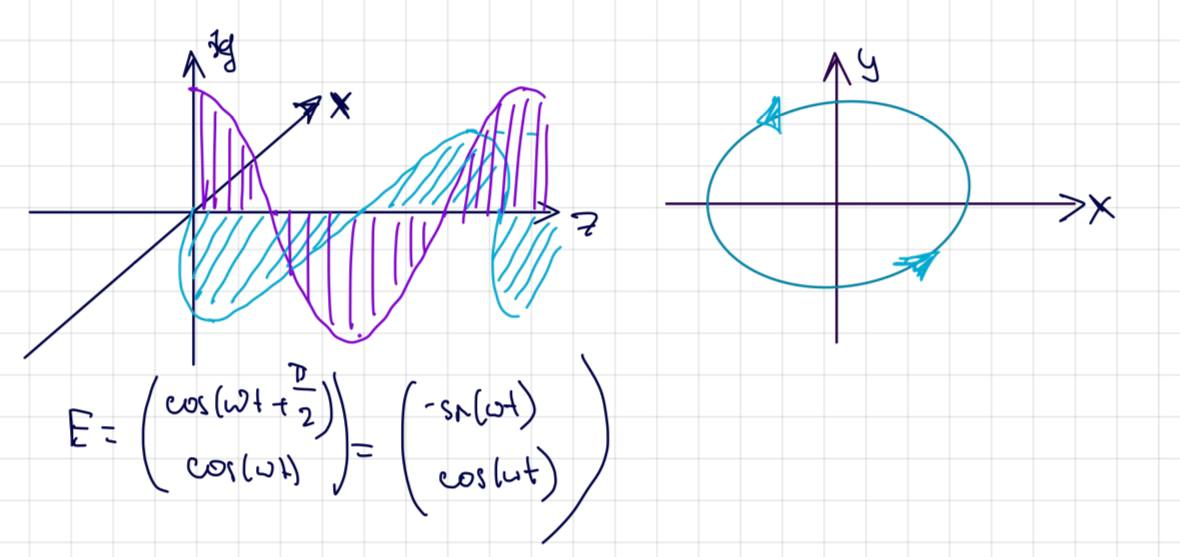
\includegraphics[scale = 0.3]{el.jpg}
    \caption{Эллипс поляризации.}
    \label{fig : 1}
\end{figure}

Направление вращения светового вектора - против часовой стрелке.
	
	Пластинку расположим между скрещенными поляроидами, после источника установим фильтр. Теперь, чтобы создать эллиптическую поляризацию, повернем первый поляроид на небольшой угол ($20^\circ$), чтобы световой вектор оказался во 2 и 4 квадрантах. Теперь параллельно нашей пластинке установим другую (тоже $\lambda/4$), у которой заранее определили главные оси.
	
	Теперь, с помощью анализатора определим положение светового вектора. Он находится по прежнему во 2 и 4 квадрантах, а значит пластинки по одиночке дают эллипсы, вращающиеся в разные стороны.
	



\section{Вывод}

В этой работе мы ознакомились с методами получения и анализа поляризованного света и экспериментально определили коэффициент преломления эбонита, значение которого хорошо согласуется с табличным. В ходе работы были получены следующие результаты:
\begin{itemize}
\item Определены разрешённые направления поряроидов --- для первого поляроида разрешённое направление горизонтальное, на лимбе $176^{\circ} \pm 1^{\circ}$, для второго поляроида --- вертикальная волна, на лимбе $120^{\circ} \pm 1^{\circ}$.
\item Был определен показатель преломления эбонита по углу Брюстера:
\begin{equation*}
    n = \tg{56^{\circ}} = 1,66 \pm 0,07.
\end{equation*}
Полученный результат в пределах погрешности совпадает с табличным $n = 1,6 - 1,7$.
\item Получили, что в стопе стеклянных пластинок преломленные лучи поляризованы эллиптически, а отраженные --- линейно вертикально.
\item Для двоякопреломляющих пластин определены главные направления --- минимумы и
максимумы интенсивности чередуются через $45^{\circ}$, главные плоскости пластин совпадают с разрешенными направлениями поляроидов при максимальной интенсивности. 
\item Выяснили, что из двух имеющихся пластинок первая из них --- пластинка $\lambda/2$, а вторая --- $\lambda/4$.
\item С помощью чувствительной пластинки установили ,что «быстрая» ось пластинки $\lambda/4$- это $\alpha_2^1 = 171^\circ$, а медленная, соотвтветственно, $\alpha_2^1 = 261^\circ$.   
\item При изучении интерференции поляризованных лучей было получено, что при вращении пластинки в отдельном квадратике изменяется интенсивность, а при вращении второго поляроида --- изменяется цвет;
\item Было определено направление вращения светового вектора в эллиптически поляризованной волне после пластинки $\lambda/4$: оно компенсирует разность фаз со второй пластинкой, «быстрая» и «медленная» оси которой известны. Таким образом, эллипс первой пластинки (с неизвестными осями) вращается в противоположную сторону второй, т.е. с учетом того, что у второй быстрая ось вертикальная, получаем, что у первой быстрая ось горизонтальна, а медленная, соответственно, вертикальна.
\end{itemize}


\end{document}
